\chapter{GainLayer Additional Results}\label{app:ch6:more_results}
\subsubsection{Small Kernel Ablation}
For consistency, we use the same reference network as the one introduced in the
previous chapter in \autoref{tab:ch5:cifar_tiny_arch}. Again, we run this on CIFAR-10, 
CIFAR-100 and Tiny ImageNet. 

We use the same naming technique as in the previous chapter, calling a network
`gainX' means that the `convX' layer was replaced with a wavelet gain layer, but
otherwise keeping the rest of the architecture the same. 

As we are only exploring the wavelet gain layer, and not any wavelet
nonlinearities, we come back into the pixel domain to apply the ReLU after
learning. 
This equates to the path shown in \autoref{fig:ch6:fwd_chain}b. 
I.e\. we are taking wavelet transforms of inputs, applying the gain layer and
taking inverse wavelet transforms to do a ReLU in the pixel space. In cases like
`gainA, gainB' from \autoref{fig:app6:gl_results}, we go in and out of the
wavelet layer twice.

We train all our networks for with stochastic gradient descent with momentum.
The initial learning rate is $0.5$, momentum is $0.85$, batch size $N=128$ and
weight decay is $10^{-4}$. For CIFAR-10/CIFAR-100 we scale the learning rate by
a factor of 0.2 after 60, 80 and 100 epochs, training for 120 epochs in total.
For Tiny ImageNet, the rate change is at 18, 30 and 40 epochs (training for 45 in total).

\begin{figure}[t]
  \centering
  \subfloat[CIFAR-10]{%
    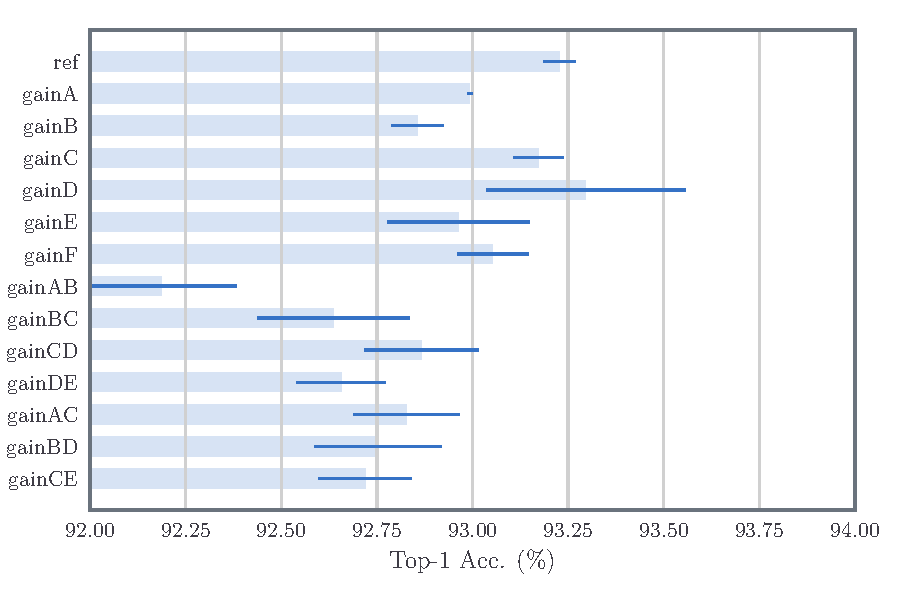
\includegraphics[width=\textwidth]{\imgpath/cifar10_gainlayer.pdf}
    \label{fig:app6:cifar10_gl}
  }\\
  \subfloat[CIFAR-100]{%
    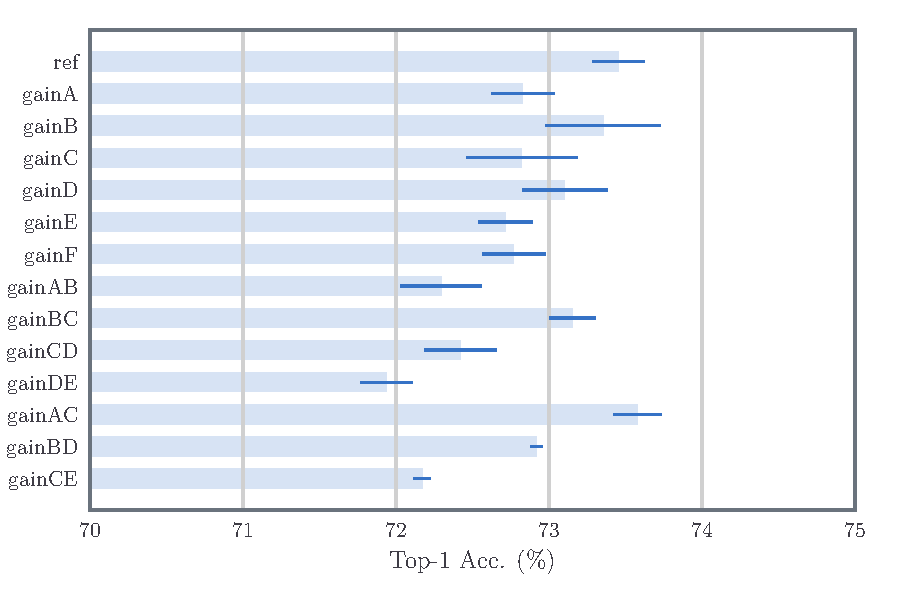
\includegraphics[width=\textwidth]{\imgpath/cifar100_gainlayer.pdf}
    \label{fig:app6:cifar100_gl}
  }
  % \subfloat[Tiny ImageNet]{%
    % 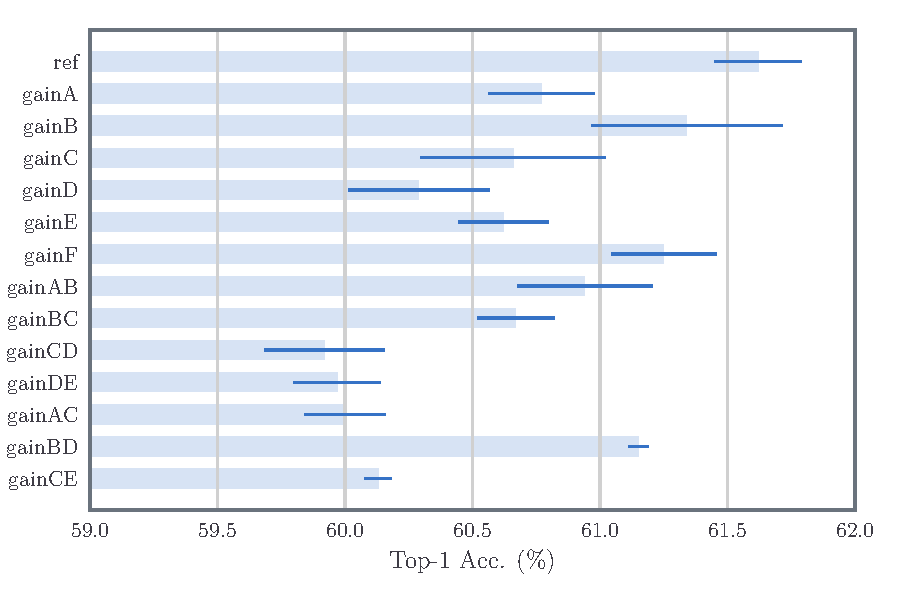
\includegraphics[width=0.8\textwidth]{\imgpath/ti_gainlayer.pdf}
    % \label{fig:ch6:ti_gl}
  % }\\
  \mycaption{Small kernel ablation results CIFAR}{}
  \label{fig:app6:gl_results}
\end{figure}

\begin{figure}[t]
  \centering
  \subfloat[Tiny ImageNet]{%
    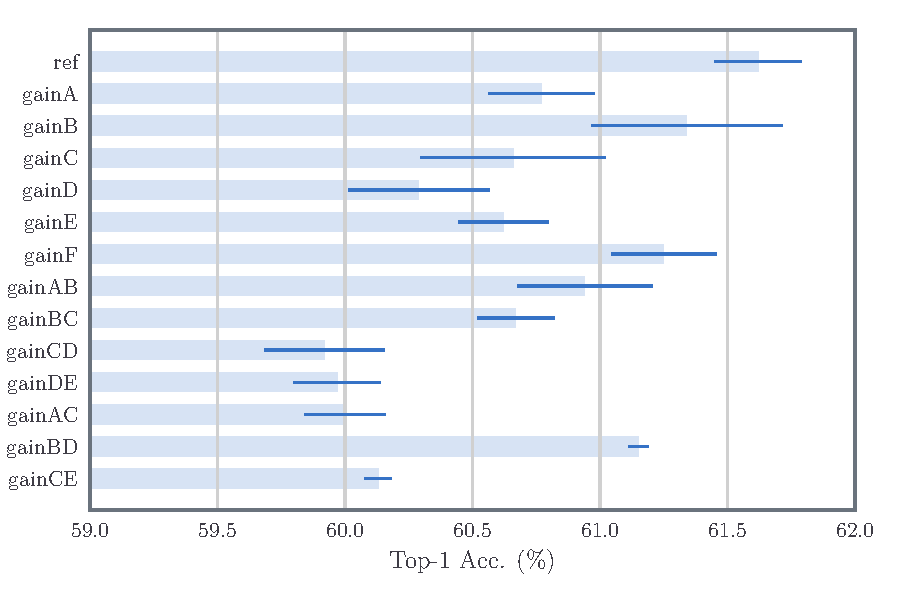
\includegraphics[width=\textwidth]{\imgpath/ti_gainlayer.pdf}
    \label{fig:app6:ti_gl}
    }
  % \subfloat[Tiny ImageNet]{%
    % 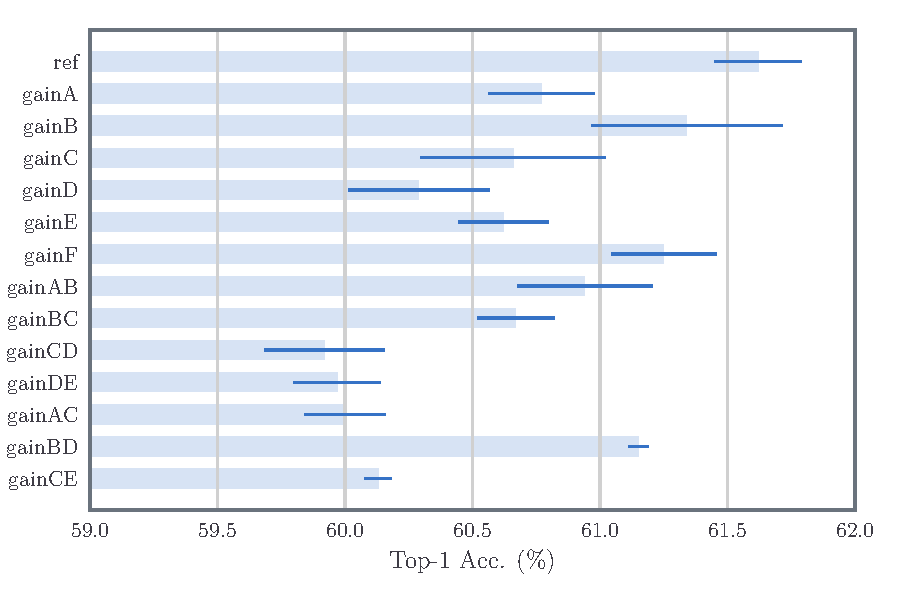
\includegraphics[width=0.8\textwidth]{\imgpath/ti_gainlayer.pdf}
    % \label{fig:ch6:ti_gl}
  % }\\
  \mycaption{Small kernel ablation results Tiny ImageNet}{}
  \label{fig:app6:gl_results}
\end{figure}

\autoref{tab:app6:ablation_results} lists the results from these experiments.
These show a promising start to this work. 
Unlike the scatternet inspired invariant layer from the previous chapter, the
gain layer does naturally downsample the output, so we are able to stack more of
them? Maybe.


